\documentclass{article}
\usepackage{ctex, graphicx, float, listings, enumitem, url, fancyhdr}
\pagestyle{fancy}
\fancyhf{}
\fancyfoot[C]{\bfseries \thepage}
\fancyhead[C]{新生研讨课报告--机器作曲}
\renewcommand{\headrulewidth}{0.4pt}
\renewcommand{\footrulewidth}{0.4pt}
\includeonly{Investigation, CompoNet, ValueNet, Toolchain, Biosphere}
\title{新生研讨课报告--机器作曲}
\author{邓胜亮\and 马凯\and 戈惊宇\and 郭金涛}
\def\allfiles{}

\begin{document}
\begin{titlepage}
\centering
\vspace*{\stretch{1}}
{\fontsize{40}{50} 机器作曲研究报告}\\
\vspace{\stretch{1}}
{\Large 邓胜亮\quad 马凯\quad 戈惊宇\quad 郭金涛}\\
\vspace{\stretch{3}}
{\today}
\end{titlepage}

\paragraph{摘要}
我们尝试利用深度学习技术以及遗传算法进行机器自动作曲,以lstm网络为基础构建模型训练了用于作曲的神经网络和用于对音符序列进行评分的神经网络,并使用后者结合遗传算法进行作曲。
\paragraph{关键词} 神经网络;遗传算法;作曲

\newpage
\renewcommand{\contentsname}{目录}
\tableofcontents

\newpage
\section{引言}
从远古时代开始直到如今,音乐贯穿了人类文明的历史,是人类用来表达情感,抒发志趣的有力工具。而善于作曲的人,往往因此而拥有一定的社会地位,被认为有着天赋的才能。于是音乐被视为了上帝的礼物,成为寄托着人类灵性的艺术。因此,普遍的看法是,音乐作为艺术,是难以由机器完成创作的。借着中国科大新生科学与社会研讨课的契机,我们小组萌生出了尝试研究机器自动作曲的想法,四人一拍即合,开始进行了尝试。本文描述了我们进行探讨的过程,并给出了我们所做的工作的相关细节,项目的全部源代码在我们的\cite{memory-lost musician}。
\section{进程}
    \subsection{提出}
    在寒假中对大数据与数据挖掘进行调研的过程中,小组成员初步了解了关于数据挖掘的相关知识。在此过程中喜好音乐的马凯同学首先提出了研究机器自动作曲的想法,小组成员表示对此很感兴趣,经过讨论之后确定了这一题目。
    \subsection{初步尝试}
    在确定这一题目后,我们经过讨论大致理清了思路。首先,考虑到音乐文件的多种格式,我们决定用较为规整、易于处理的mid文件作为训练数据来源和生成的格式。然后我们简单修改了\cite{char-rnn}训练了一个作曲网络,基本思路是根据之前的音符序列预测下一个音符。输入一些音符就可以得到一首曲子。

    初步尝试前,我们编写了爬虫收集到大约2000个mid文件,完成了网络上有关信息的收集、了解了世界上已有的一些在研究机器自动作曲的团队的思路、成果和遇到的问题,并完成了模型的初步构建。

    在此次尝试中,我们利用软件\cite{jmusic}对mid文件进行初步处理,得到由不同音轨多个note组成的xml文件,每个note包含四个要素:pitch,dynamic,rhythmValue,duration。由于jmusic文件说明的缺失,我们并不完全清楚这四个要素的含义,于是先选取了可能代表音高和持续时间的rhythmValue和duration构建二维向量。将前述向量简单处理为字节序列作为训练数据输入模型进行训练。训练出作曲网络后,我们用人工输入的音符作为初始音符生成了一些片段。

    在结果中,我们不时能听到一小段悦耳的音乐,但是大多数时候都是缺乏基本乐理的混乱音符。初次尝试的主要收获是验证了工具链的可用性。初次尝试的结果虽然不佳,但是我们产生了一些新的想法,例如将训练数据进一步处理、寻找主音轨、转换方向利用遗传算法进行研究等。
    \subsection{反复修改}
    初步尝试结束之后,我们进行了更多的细化工作,比如完善工具链、收集更多数据等。同时,我们根据初步尝试的结果与新想法完成了一些工作。在这段时间里,我们通过尝试,弄清了四个要素的含义,并借助于此,绕开寻找主音轨的困难直接处理多音轨的音乐。

    在此次尝试中,我们将多音轨重排成顺序排列的音符,将四个音符要素进行one-hot编码,再连接成一个向量作为神经网络的输入。效果见\ref{result_of_CompoNet}。
    \subsection{想法的突破与实现的失败}
    此前的模型使用均方差或\cite{交叉熵}作为损失函数,其本质上都是在让神经网络的输出更接近已经有的音乐。随着工作的推进,我们慢慢感到其不足之处。于是我们产生了一个新想法--能不能训练出一个专门用来打分的神经网络,并基于它设计损失函数?有了这样一个用于打分的模型,我们能更好的告诉机器“什么是音乐”,能够在曲风和情感上进行选择,最关键的是能够让机器从原本的模仿改变成真正的创作。于是我们基于卷积神经网络实现了一个评分网络。实现之后我们发现,技术上似乎做不到将神经网络的输出作为损失函数(和求梯度、随机取样过程有关),于是我们将这个神经网络用在了遗传算法的适应度评估中。

\section{调研成果}
经过调研,我们知道目前有六个较大型的机器自动作曲项目,下面进行简单的分析。
    \subsection{Magenta}
    Magenta是Google的一个开源的深度学习音乐生成项目。该项目在2016年6月开源,目前实现了一个基于常规RNN的模型和两个LSTM的模型。

    它可以处理任何单声道mid文件,其团队正在积极改进模型并增加功能。对于每个模型,Magenta已经提供了一个训练捆绑包,其中有数千个mid文件,可以直接使用这些预先训练的模型生成新的mid文件。

    但是Magenta只能生成单个音符流,也就是说其生成的音乐只能是单音轨的,他们正努力将生成的旋律通过人为的加上鼓点或吉他,但是到目前为止仍未真正解决这一问题。

    其github网址如下

    \url{https : //github.com/tensorflow/magenta}

    \subsection{DeepJazz}
    Deepjazz是Ji-Sung Kim在一次hackathon(编程马拉松)中用36小时完成的作品。它处理的对象同样是mid文件,其模型是一个两层的LSTM。

    它可以通过在单个mid文件上进行训练来创建一些爵士乐,它先将一个mid文件遍历多次,然后可以进行创作。

    不同于Magenta,它可以处理和弦。但它其实是将爵士乐转换成单乐器和单音轨,最后生成的音乐同样是单乐器、单音轨的。

    其github网址如下

    \url{https : //github.com/jisungk/deepjazz}

    \subsection{BachBot}
    BachBot是剑桥大学Feynman Liang团队的成果。它面向的是巴赫的音乐,主体模型同样是LSTM。

    它创造的巴赫的音乐几乎可以以假乱真,而且它可以处理多达4个声道的声音。

    如果给BachBot一个声道的声音,它可以很完美的补上三个声道,从而形成一首完美的曲子,但是如果不这样做,它的表现就差强人意了。

    \subsection{FlowMachines}
    FlowMachines是索尼旗下的一个团队的作品。他所使用的神经网络技术是Markov constraints。

    目前为止,它通过“分析”近 13000份世界各地不同风格的乐谱(主要是爵士乐和流行音乐也有很多巴西音乐、百老汇和其他音乐风格),在人类作曲家协助下完成了一首披头士风格的流行音乐制作。

    但是,在音乐生成的过程中音乐家的工作是不可或缺的,也就是说,并不是常人点击一个按钮就可以创造音乐。

    \subsection{WaveNet}
    WaveNet是Google DeepMind的研究人员所创建的项目。WaveNet主要基于卷积神经网络。需要说明的是,该项目的目的并不是机器自动作曲,它的主要目的是通过训练使得机器能更更好的完成文本转语音功能,但其基本原理仍然是输入音频和输出音频。

    不同于以上的几个项目,WaveNet的输入并非音符数据而是原始音频,于是也就不存在有关音轨的问题,它可以产生任何种类的声音。

    由于原始音频数据量之庞大,该算法计算上十分昂贵,需要几分钟的时间来训练一秒钟的声音。

    \subsection{GRUV}
    GRUV是斯坦福的一个研究项目,它同样采用原始波形作为输入。其神经网络技术基于LSTM和GRU。

    GRUV是世界上最早的一个公布的以原始波形作为输入的自动作曲项目,它以Madeon的歌曲作为训练数据,并成功生成了一些歌曲。

    GRUV面临着与WaveNet同样的问题,并且该项目研究人员没有时间和计算能力进行进一步研究,该项目受制于硬件和软件两方面的原因没有更进一步。

    其github网址如下

    \url{https://github.com/MattVitelli/GRUV}

    \subsection{小结}
    我们可以看到,这几个项目主要分为以音符数据为输入和以原始波形为输入的两类。在以音符数据为输入的一类中,无一例外的遇到了关于多音轨处理的问题;而在原始波形这一类中,大多受制于昂贵的计算成本和硬件需求。这两类中,音符类的计算复杂度要低得多,但是相应的,其生成音乐的复杂性也不能向后者那样达到与整个语料库的组合同等复杂,仅仅只能达到与语料库中的单曲同等复杂。

    还有一个问题是,目前为止的几个结果中,生成音乐时,都需要作曲家的协助,并非简单地点击按钮就可以得到想要的音乐,这与我们最初的期望还相去甚远。
 

\documentclass[UTF8]{ctexart}
  \title{关于工具链}
  \author{邓胜亮}
  \email{faultrit@outlook.com}
\begin{document}
  \maketitle
  \section{功能}
    我们编写了一套工具来将mid格式的音乐转换为我们需要的格式。
\end{document}

\documentclass{article}
  \title{关于}
  \author{邓胜亮}
  \usepackage{ctex, graphicx, float}
\begin{document}
  \section{功能}
    接受一段音符序列,对其进行“续写”。
  \section{输入}
    我们在已有的mid文件中随机选取了一些统计了音符的四个要素
    (pitch,dynamic,rhythmValue,duration)的分布情况如图1,2,3,4:
    \begin{figure}[H]
      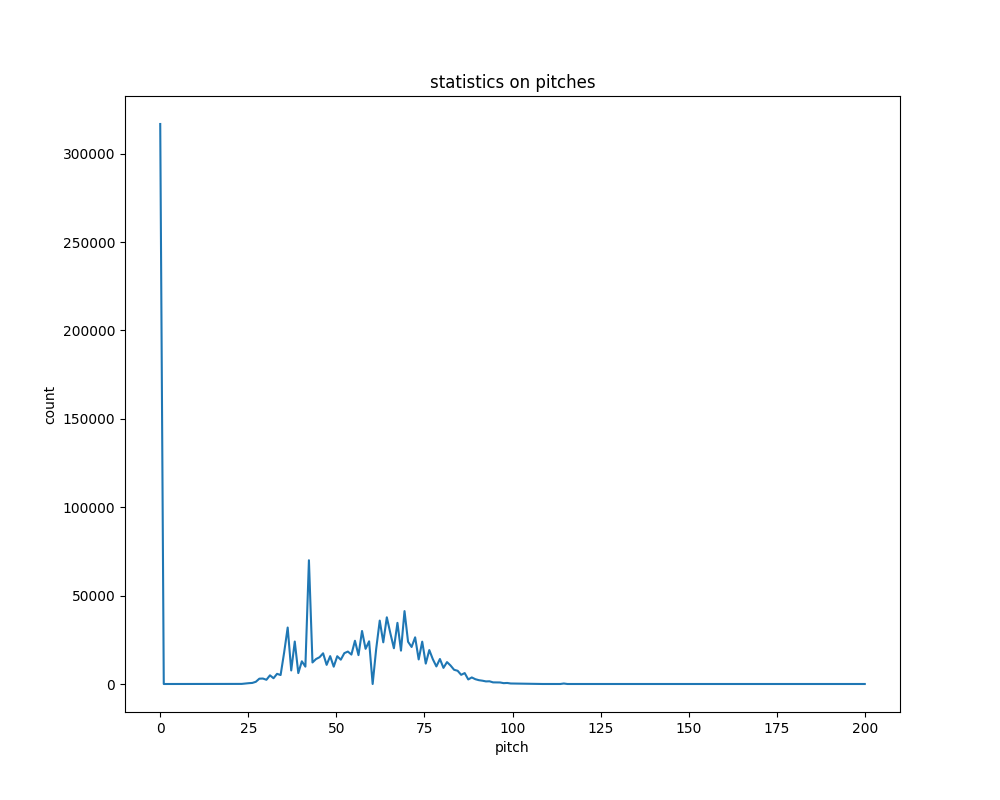
\includegraphics[width=.5\textwidth]{picture/pitches.png}
      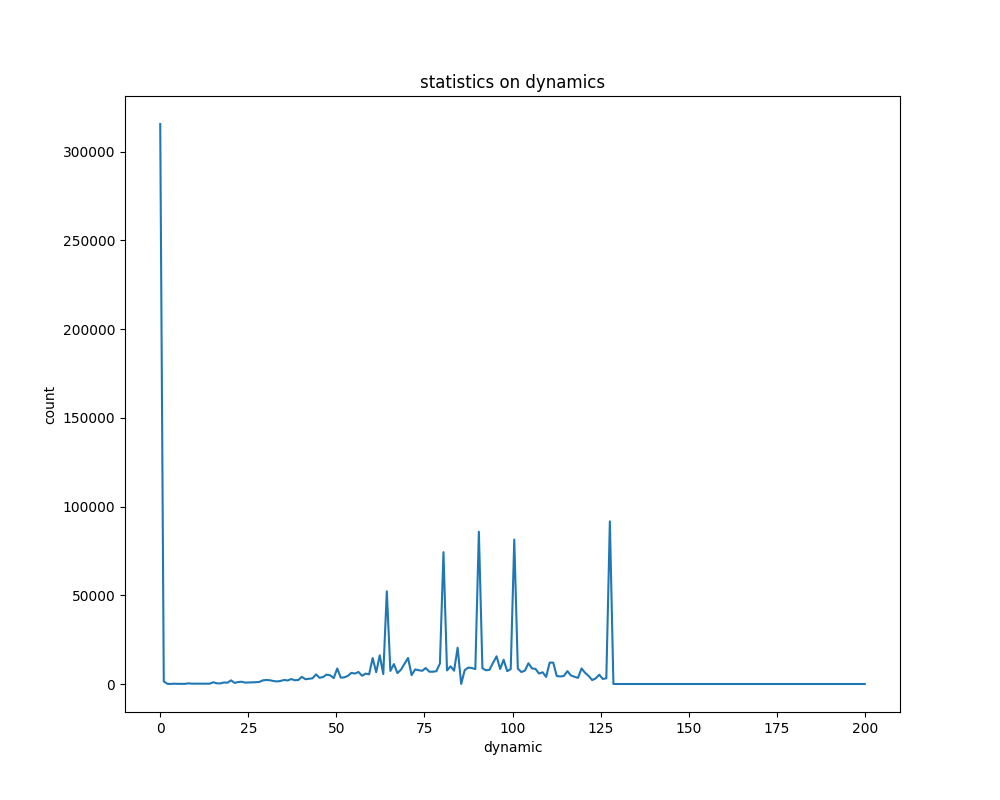
\includegraphics[width=.5\textwidth]{picture/dynamics.png}
      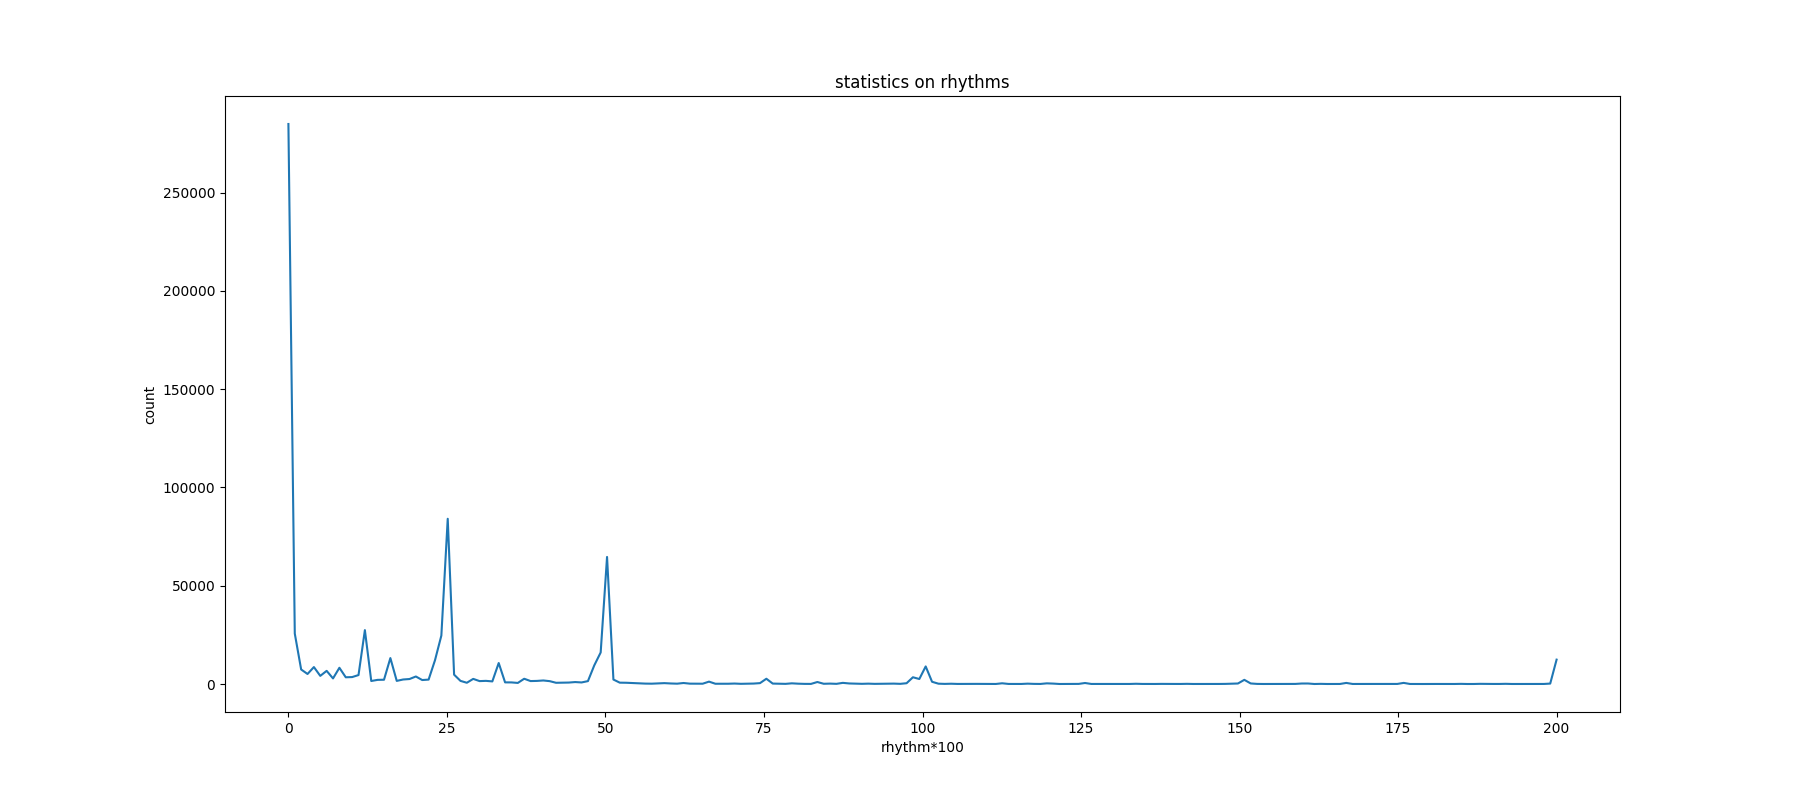
\includegraphics[width=.5\textwidth]{picture/rhythms.png}
      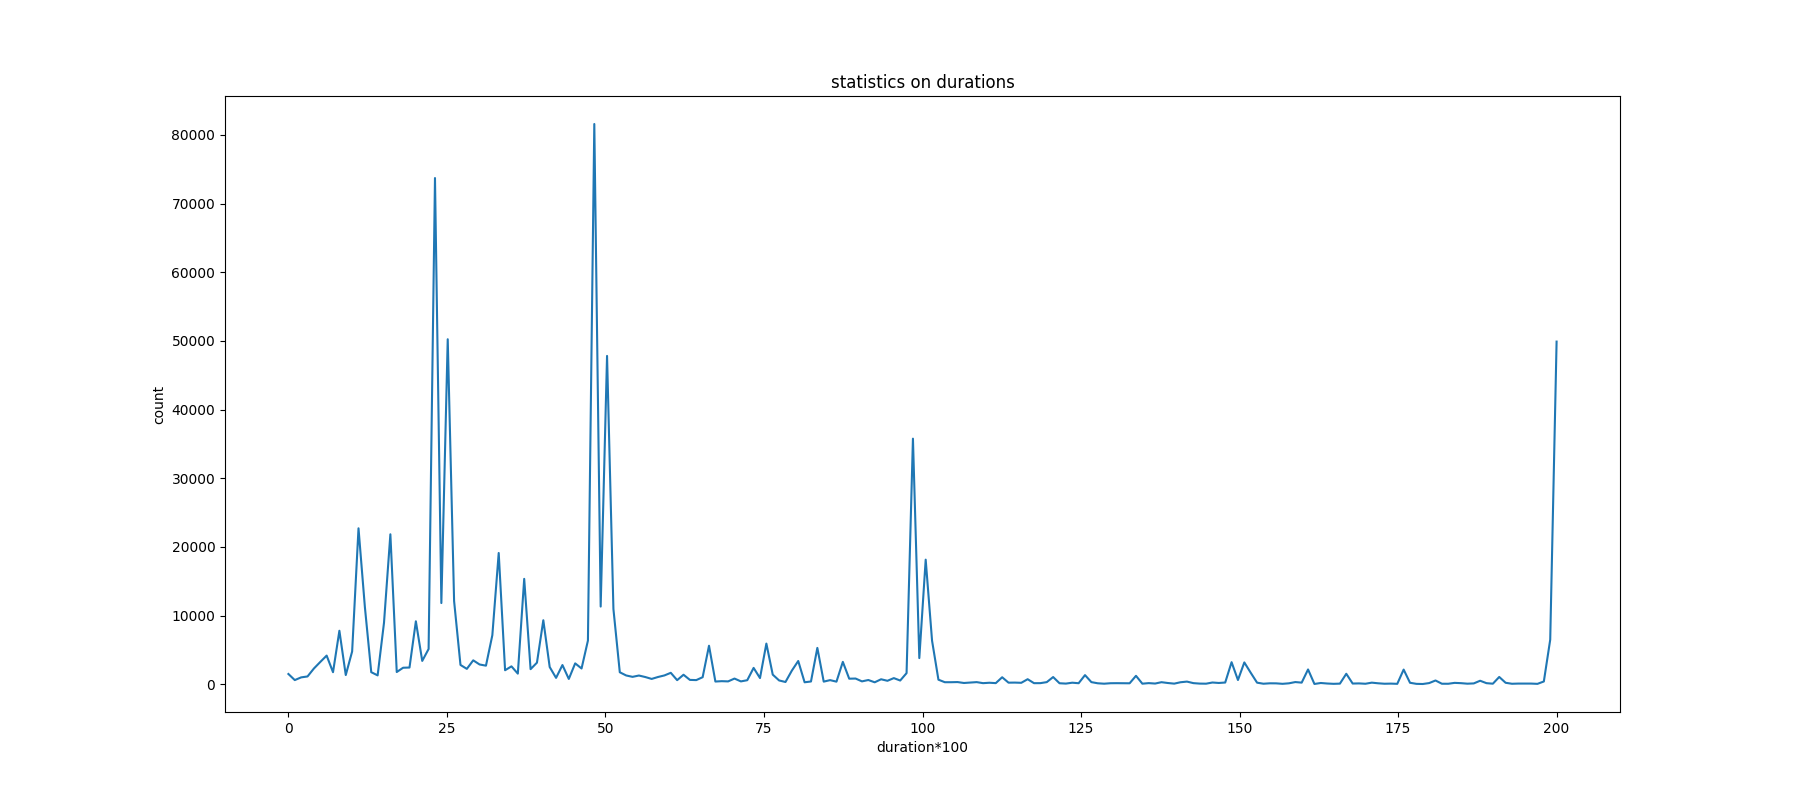
\includegraphics[width=.5\textwidth]{picture/durations.png}
    \end{figure}
    可以看出,虽然rhythmValue和duration的取值理论上是连续的,但实际上取到的值很有限,
    因此可以认为这四个要素都是离散的。基于这个事实,
    为了能够进行随机取样和关于“信息密度”的直觉判断,
    我们对输入的四个要素先分别进行one-hot编码,再连接成一个向量作为神经网络的输入。

  \section{结构和训练}
    我们模仿char-rnn-tensorflow构建了一个两层、每层128个神经元的lstm,增加了一个隐层
    将lstm层的输出变换为和输入向量相同的长度,然后拆分为四个部分,对每部分计算softmax,
    得到音符的每个要素所有取值的概率分布,然后将其与下一个音符的one-hot编码计算交叉熵作为
    损失函数。
  \section{效果}
\end{document}

\documentclass[UTF8]{article}
  \title{关于}
  \author{邓胜亮}
  \email{faultrit@outlook.com}
\begin{document}
  \maketitle
  \section{功能}
    对一段给定的音符序列打分\footnote{},衡量其是“我们所倾向的音乐”的程度。
  \section{目的}
    设计这个神经网络的最初目的
    是用来代替作曲网络(CompoNet)原来的cost函数,使训练目标更接近于“是音乐”而不是
    “和训练用的音乐一致”,但后来发现受到技术的限制,我们无法完成这种替换,于是又想到可以
    把它作为遗传算法的适应度计算函数。
  \section{输入}
    为了避免音符四个要素的数值大小差别太大造成的问题,基于统计出的四个要素的数值分布,
    我们设计了四个压缩函数来将四个要素的数值分别映射到0到1之间。
    \subsection{压缩pitch与dynamic}
      对于pitch和dynamic的压缩基于sigmoid函数,因为这两者的分布比较集中于某个
      中间值,而sigmoid函数在中间部分很陡峭,适合将“密集”的值分散开。
      压缩前后的分布如下:
      \includegraphics{}
      \includegraphics{}
    \subsection{压缩rhythmValue与duration}
      对于rhythmValue和duration的压缩基于对数函数,因为它们的原始取值的分布呈先密集后
      稀疏的特点,而对数函数先陡峭后平缓,有助于使压缩后的分布趋于均匀。
      压缩前后的分布如下:
      \includegraphics{}
      \includegraphics{}

  \section{结构和训练}
    我们使用了卷积神经网络(CNN)而不是擅长处理序列的递归神经网络(RNN),原因是我们
    认为音乐具有相当强
    的局部特征,利用CNN的卷积层和池化层可以提取其局部特征\cite{},而提取后的
    局部特征在全连接层被处理又有一种“考虑全曲的情感变化”的感觉,因此我们觉得这很适合用
    CNN来处理。
    输入是一维的,有四个channel(即音符的四个要素)。
    第一层为卷积层,感受野宽度为8,卷积核数为8。
    第二层为池化层,池化方式为最大池化,池化宽度为4。
    第三层为卷积层,感受野宽度为4,卷积核数为16。
    第四层为池化层,池化方式为最大池化,池化宽度为8。
    第五层为全连接层,输出为一个数值,我们将它视作该网络对输入序列的评分。

    我们手工对一些曲子进行了打分,分为1.0、0.6、0.4、0.0,1.0主要是莫扎特的作品,
    0.6和0.4是凭感觉在已有的midi文件中选出来的,0.0是随机生成的。
  \section{效果}
    在训练了足够长的时间后,我们在训练数据上进行了评分效果的评估\footnote{},将网络的输出
    与给出的标签差距小于0.1的视为正确,正确率如下:
      % TODO
    经过抽样对比神经网络评分与标签的差别,我们发现虽然有时误差大于0.1,
    但神经网络给出的评分还是比较准确的。 % TODO
\end{document}

\documentclass{ctexart}
\usepackage{listings}
\usepackage{enumitem}
\begin{document}

\section{Biosphere技术细节}
Musinet的遗传算法部分称作Biosphere(生物圈)。

Biosphere的基本流程与一般GA相同,即将信息编码后放在一起作为种群,
然后依次对这个种群实施基因突变、选择复制、交配得到下一代。

\subsection{信息表示}
Musinet把一个乐谱表示为如下Python数据结构:
\begin{lstlisting}
note = [pitch, dynamic, rhythm, duration]
notes = [note]
part = [instrument, notes, rank]
score = [part]
\end{lstlisting}
GA只使用长度为512的notes,即一个染色体是长度为512的列表,列表元素是长度为4的列表。

\subsection{适应度与自然选择}
GA的适应度函数直接使用打分网络(ValueNet)的输出。其基本考虑是,CNN可能在识别音乐特征上比RNN更有优势。

自然选择的过程使得种群的整体适应度提升,自然选择后种群就为交配做好了准备。
Biosphere使用了简单了轮盘赌算法。流程如下:
\begin{enumerate}[nosep]
  \item 将每个个体的适应度相加得到$T$
  \item 任取$[0,T]$之间的随机数$M$
  \item 令$S$等于前$i$个个体的适应度,且$S$恰好不小于$M$
  \item 把第$i$个个体放入交配池
\end{enumerate}

\subsection{杂交算子}
Biosphere使用了简单的单点片段交换算法,流程如下:
\begin{enumerate}[nosep]
  \item 取种群中$P_c$比例的个体进行交配,其余个体复制到下一代
  \item 对于任意一对个体A、B,任取一个位点$i$,使得A和B的染色体恰互换$i,i+\mathrm{gene\_len}$之间一段
  \item 把得到的两个新染色体放入下一代
\end{enumerate}

\subsection{效果评估}
经过多轮测试、试听多个产生的ValueNet认为足够好(适应度 > 0.9)的曲子后,我们发现生成的效果不好:和随机产生的曲子差别不大。
GA方法基本是失败的。

可能的原因:
\begin{enumerate}[nosep]
  \item 参数$P_m,P_c$设置不当,导致种群不能稳定收敛
  \item 选择算法过分简单,不能保存优良基因、淘汰不良基因
  \item 杂交算法未充分考虑音乐特性,不能有效交换优良基因
  \item ValueNet不能真正把好音乐选出来
\end{enumerate}

我们就以上原因进行了改进实验,但均未获得良好效果。
推测是以上原因中一个或多个导致搜索效率过低,或者无法收敛到我们寻求的音乐。

\end{document}


\section{总结}
虽然我们的成果并不太好,CompoNet产生的比较好听的音符序列几乎是在背诵训练数据,ValueNet并不能真正地识别音乐,Biosphere受到ValueNet的限制在随机初始种群的条件下筛选出的高分“音乐”其实没法听,但在这次尝试中,我们所有人都得到了团队合作能力和解决问题能力的提高,也学到了许多关于机器学习、数据挖掘方面的知识,收获很大。

\begin{thebibliography}{}
\bibitem[github仓库]{memory-lost musician} \url{https://github.com/faultrit/memory-lost-musician}
\bibitem[char-rnn]{char-rnn} \url{https://github.com/karpathy/char-rnn}
\bibitem[jmusic]{jmusic} \url{http://explodingart.com/jmusic/}
\bibitem[交叉熵]{交叉熵} \url{https://en.wikipedia.org/wiki/Cross_entropy}
\end{thebibliography}

\end{document}
